\documentclass[11pt,english]{article}
\usepackage{listings}
\usepackage{amsmath}
\usepackage{graphicx}
\usepackage{morefloats}
\usepackage[toc,page]{appendix}
\graphicspath{ {../} }

\author{Sean Curran \\
\and Stephen Durofchalk \\
\and Zachary Feldman \\
\and Ryan Wails}

\title{EE454 Project 1 Report}
\lstset{language=Matlab}
\renewcommand{\thesection}{\alph{section}}

\begin{document}
\maketitle

\newpage
\section{Project Summary}

\section{Procedural Approach}

\section{Experimental Observations}

\subsection{Intermediate Output}

Intermediate output generated by the CNN is included in the appendix attached to this report.  Each figure shows the concatenated output of each layer as a gray scale image.  The images can be produced by running `demo.m.'

Observation of the output from each layer is consistent with the project description.  Normalization produces an image with scaled pixel values but is relatively unchanged.  Convolution produces a set of images with different feature sets extracted.  The ReLu produces an image with a 0 threshold (MATLAB's imagesc command slightly changes the output image because the range of the pixel values in the image changes).  Max Pooling reduces the size of the image by a factor of (nxn) and has the effect of making the previous image look more ``blocky'' via down-sampling.  Finally, we have the fully-connected layer and the soft max layer which produce a vector of classification probabilities from the image which are represented by the bar graph.

\section{Performance Evaluation}
\subsection{Results}
	The following results were the outcome of classifying images as the class associated with the highest probability in the probability vector.
\begin{center}
	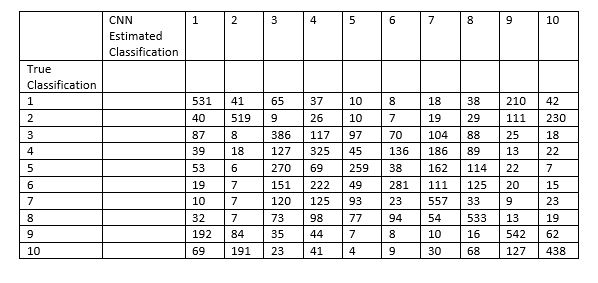
\includegraphics[scale=0.8]{confusionmatrix}
	~\\~\\
	
		\textbf{Accuracy = 43.7\%}
\end{center}


\begin{center}
	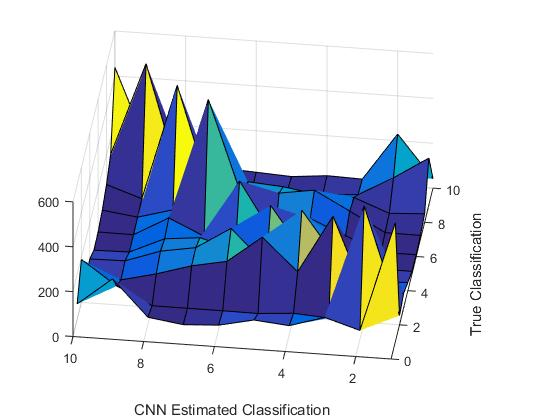
\includegraphics[scale=0.7]{confsurf}
	~\\~\\
\end{center}
\textbf{Discussion:}

	
   The surface plot above demonstrates how well the CNN classifies images. There is a very strong response on the diagonal which represents the correct classifications. What is interesting is that this matrix is somewhat diagonal. This demonstrates that if images in a class of images $C_1$ are being confused for images in a class of images $C_2$, then images in $C_2$ are also being confused for images in $C_1$. A lot of this confusion is entirely logical; for example, trucks and automobiles are frequently confused for each other. Another great example of confusion are cats and dogs are frequently confused for one another. We are again very impressed with how well the CNN because it not only detects similarities between images within a class, but it detects similarities amongst images spanning multiple classes.
       
    ~\\
    \noindent
    Note: The above results were produced using NeuralNet function located in 'NeuralNet.m'.

\subsection{Looking at the Top-k Highest Probabilities}
	The following subsection looks at how frequently an image's true class appears in one of the top-k ranked classes, as determined by probability scores sorted from highest to lowest.
\begin{center}
	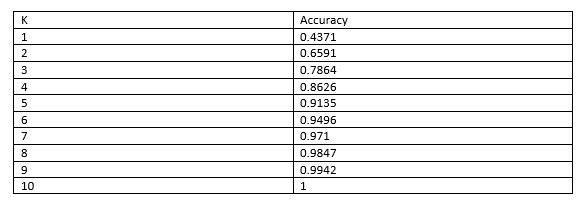
\includegraphics[scale=0.8]{topktable}
	Note: Accuracy is the percentage of times that the correct object class appeared in the top-k ranked classes, as determined by probability scores sorted form highest to lowest. 
	~\\
\end{center}
\begin{center}
	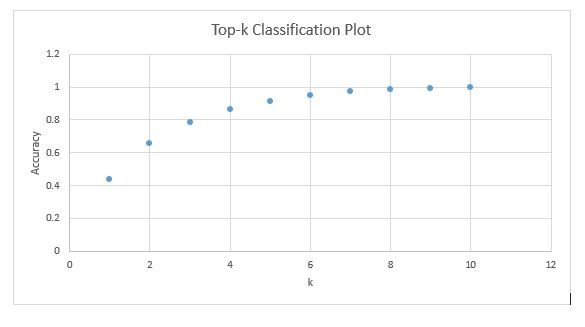
\includegraphics[scale=0.8]{topkplot}
	~\\~\\
\end{center}
\textbf{Discussion:}
      We were very surprised to see the top-k classification plot follow an exponential distribution. This demonstrates that the probability estimations provided by the CNN are accurate. We expected the probability estimations to be an arbitrary metric, but looking at the logarithmic nature of the plot it is clear that the probabilities are very accurate. 

	~\\
	\noindent
	Note: The above results were produced using the topk function located in 'topk.m' and NeuralNet function located in 'NeuralNet.m'.

\section{Further Exploration}
\subsection{Test Cases}
To test the robustness/accuracy of the training outside of the given data set, additional test images were gathered and fed into the CNN.  Images were rescaled to thumbnail size (32x32x3) with the Matlab command
\begin{lstlisting}
thumbnail = imresize(img, [32 32]);
\end{lstlisting}

\noindent
110 images total were collected; 100 fell into the preexisting image classes, 10 contained scenes not falling into any preexisting class.  Running these new 10 images through the CNN yielded the following results:\\

\begin{tabular}{ | c | c | c |}
  \hline
  Image \# & Image Contents & CNN Classification \\
  \hline		
  Image 1 & Tree in Field & Horse (8) \\
  Image 2 & Winter Mountain Scene & Ship (9) \\
  Image 3 & Ryan and Zach & Bird (3) \\
  Image 4 & Steve & Frog (7) \\
  Image 5 & Sean & Cat (4) \\
  Image 6 & Desktop Computer & Automobile (2) \\
  Image 7 & Football on Field & Deer(5) \\
  Image 8 & Robert Collins & Truck (10) \\
  Image 9 & Old Main & Bird(3) \\
  Image 10 & Penn State Logo & Truck (10)\\
  \hline  
\end{tabular}

\subsection{Reclassification}
An attempt was made to distinguish these 10 images from the rest of the data set (i.e. reclassify these 10 images as unknown).  Let $V$ be the vector of output probabilities from the CNN for each image.  Let $C$ be the classification of the image producing probability vector $V$.  Originally, we have\\~\\
\begin{math}
p_i \in V \\
p_{max} = \max(p_1, p_2,...,p_{10}) \\
C = i $ given $ p_i = p_{max}
\end{math}

~\newline\noindent
To reclassify the images we use\\
\noindent
\begin{math}
p_{max} = \max(p_1,p_2,...,p_{10}) \\
P = \{p_1,p_2,...,p_{10}\} \setminus \{p_{max}\} \\
p_{2max} = \max(P) \\~\\
\begin{cases}
C = i $ given $ p_i = p_{max} & $for	$ p_{max} - p_{2max} >= 0.25 \\
C = 11 & $otherwise$
\end{cases}
\end{math}
~\\~\\
Less precisely, the difference between the two peak responses was thresholded by .25; so, if there were two strong responses, the image is reclassified as unknown.

\subsection{Results After Reclassification}
In the confusion matrix below, classes 1 through 10 are the same classifications.  Class 11 identifies an unknown image class. \\\\
\begin{tabular}{ | c | c | c | c | c | c | c | c | c | c | c | c | c | }
\hline
	 & CNN
Class & 1 & 2 & 3 & 4 & 5 & 6 & 7 & 8 & 9 & 10 & 11 \\ \hline
	True 
Class &  &  &  &  &  &  &  &  &  &  &  &  \\ \hline
	1 &  & 3 & 0 & 0 & 0 & 0 & 0 & 0 & 0 & 1 & 0 & 6 \\ \hline
	2 &  & 1 & 2 & 0 & 0 & 0 & 0 & 0 & 0 & 2 & 0 & 5 \\ \hline
	3 &  & 1 & 0 & 2 & 0 & 0 & 0 & 0 & 0 & 0 & 0 & 7 \\ \hline
	4 &  & 0 & 0 & 0 & 1 & 0 & 0 & 0 & 0 & 0 & 0 & 9 \\ \hline
	5 &  & 0 & 0 & 0 & 0 & 0 & 0 & 0 & 1 & 0 & 0 & 9 \\ \hline
	6 &  & 0 & 0 & 2 & 0 & 0 & 0 & 0 & 0 & 0 & 0 & 8 \\ \hline
	7 &  & 0 & 0 & 0 & 1 & 0 & 0 & 1 & 0 & 0 & 0 & 8 \\ \hline
	8 &  & 0 & 0 & 1 & 1 & 0 & 0 & 1 & 4 & 0 & 0 & 3 \\ \hline
	9 &  & 0 & 0 & 0 & 0 & 0 & 0 & 0 & 0 & 5 & 0 & 5 \\ \hline
	10 &  & 0 & 0 & 0 & 0 & 0 & 0 & 0 & 0 & 0 & 5 & 5 \\ \hline
	11 &  & 0 & 0 & 0 & 0 & 0 & 0 & 0 & 0 & 1 & 0 & 9 \\ \hline
\end{tabular}

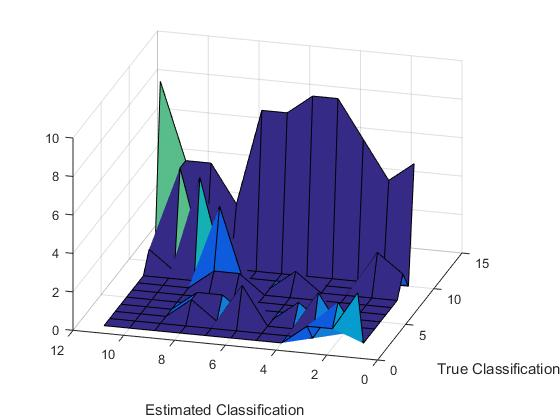
\includegraphics[scale=0.6]{confexp}
~\\~\\
\textbf{Accuracy = 29.09\%}
\\
The reclassification metric does well in replacing the 10 new images in the unknown category, but also places images that were previously correctly classified in the unknown category.  Other metrics tested were
\begin{enumerate}
\item Thresholding on the number of classes that had a response above 0.1 (the mean value for random classification)
\item Taking the spatial derivative of the probability vector; this metric actually produces zero-mean Gaussian noise with a very small standard deviation.
\end{enumerate}

\section{Member Contributions}

\newpage
\begin{appendices}
\section{Intermediate Output}

\begin{figure}[h!]
  \caption{Original Image}
  \centering
    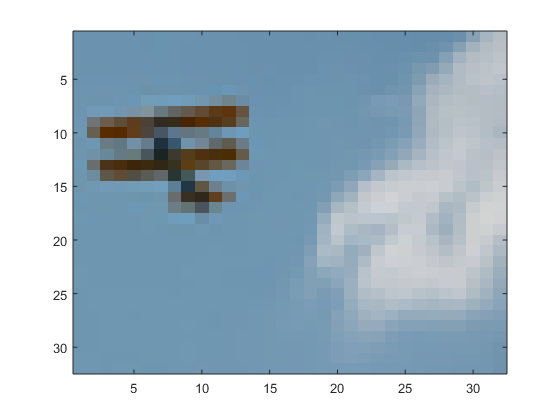
\includegraphics[width=0.75\textwidth]{layer/0}
\end{figure}

\begin{figure}[h!]
  \caption{Layer 1 Output}
  \centering
    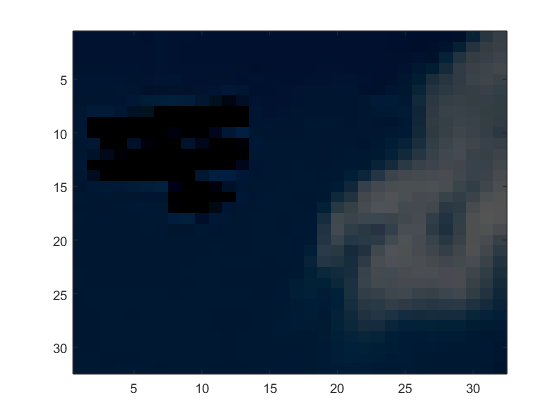
\includegraphics[width=0.75\textwidth]{layer/1}
\end{figure}

\begin{figure}[h!]
  \caption{Layer 2 Output}
  \centering
    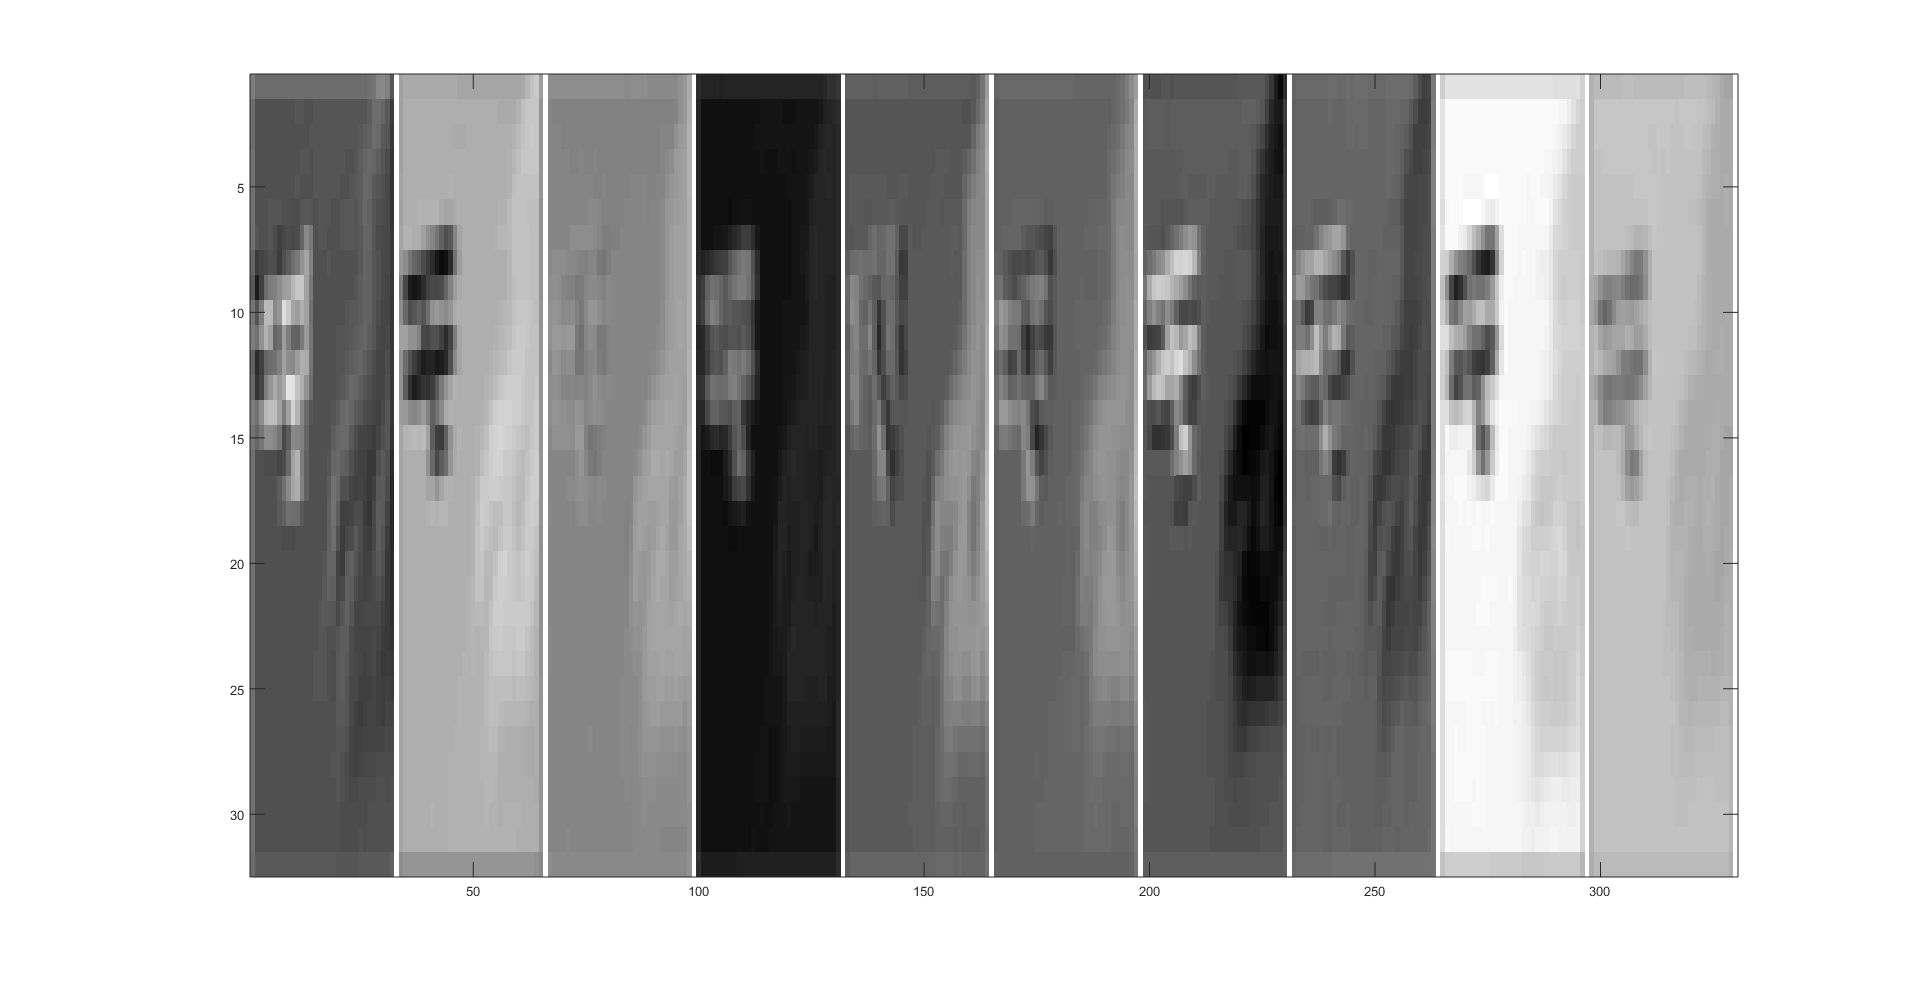
\includegraphics[width=\textwidth]{layer/2}
\end{figure}

\begin{figure}[h!]
  \caption{Layer 3 Output}
  \centering
    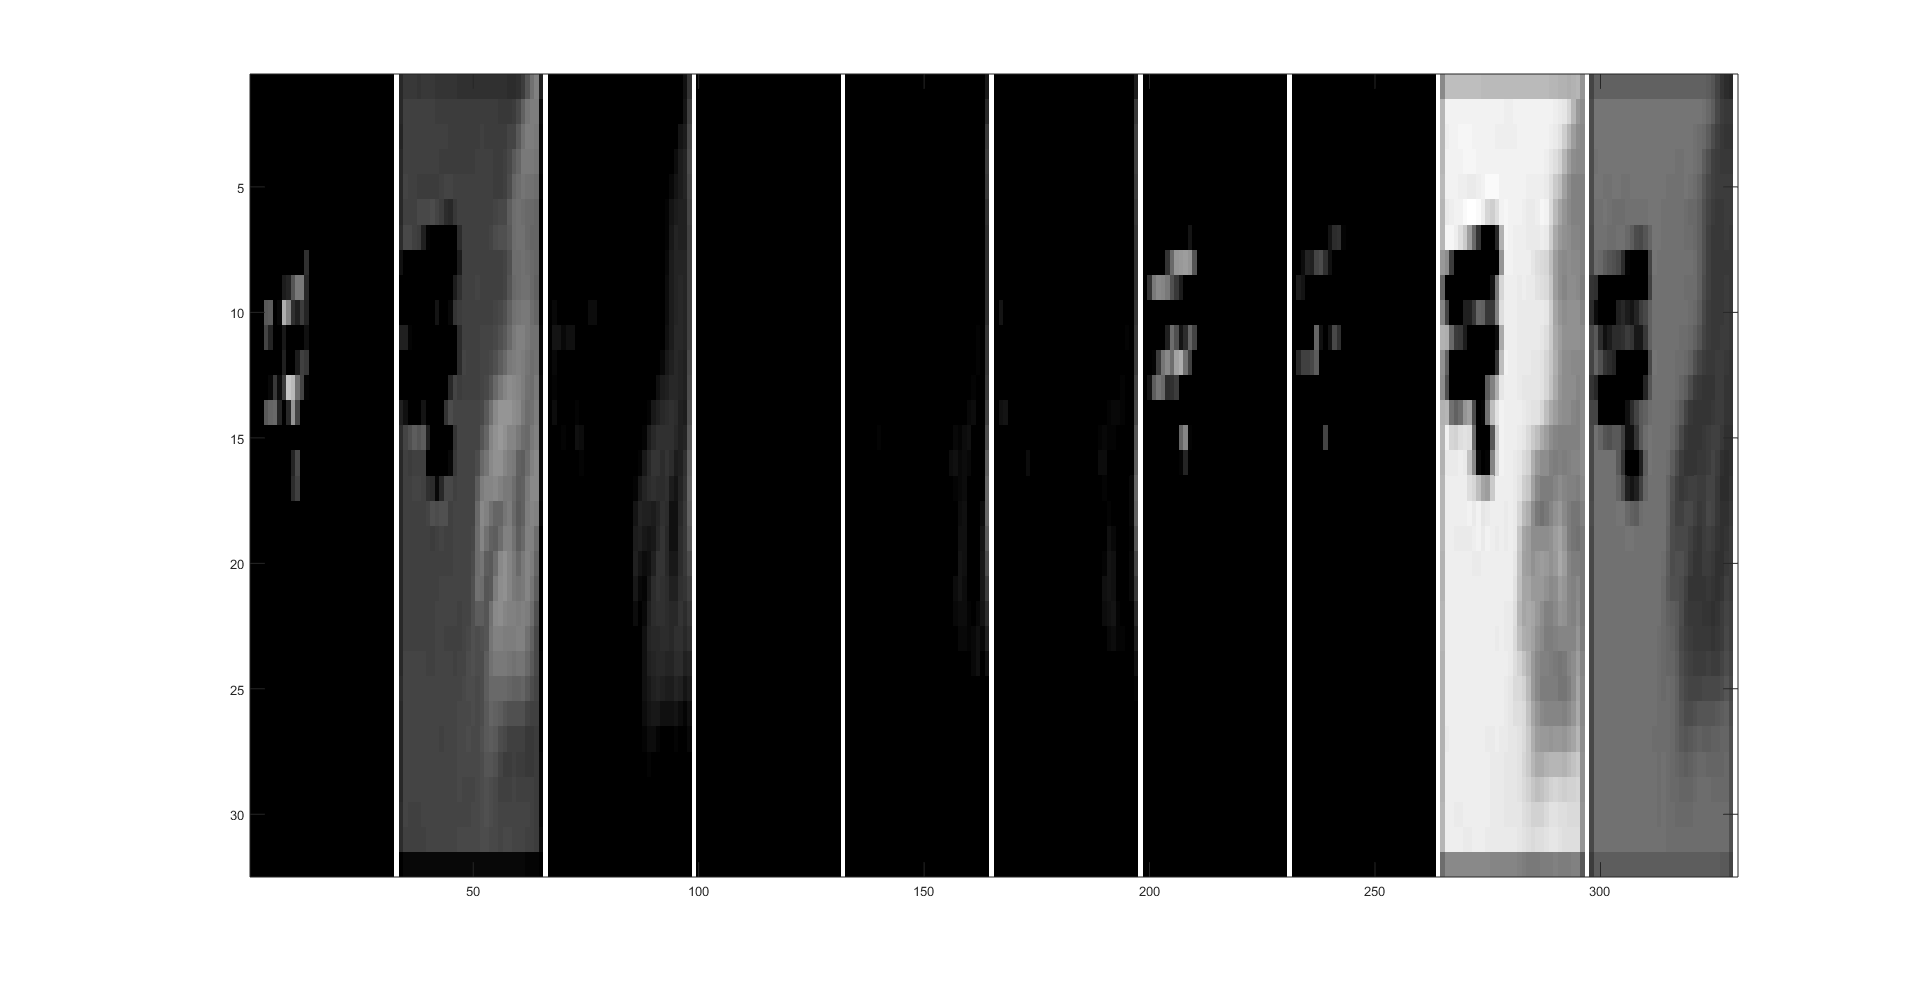
\includegraphics[width=\textwidth]{layer/3}
\end{figure}

\begin{figure}[h!]
  \caption{Layer 4 Output}
  \centering
    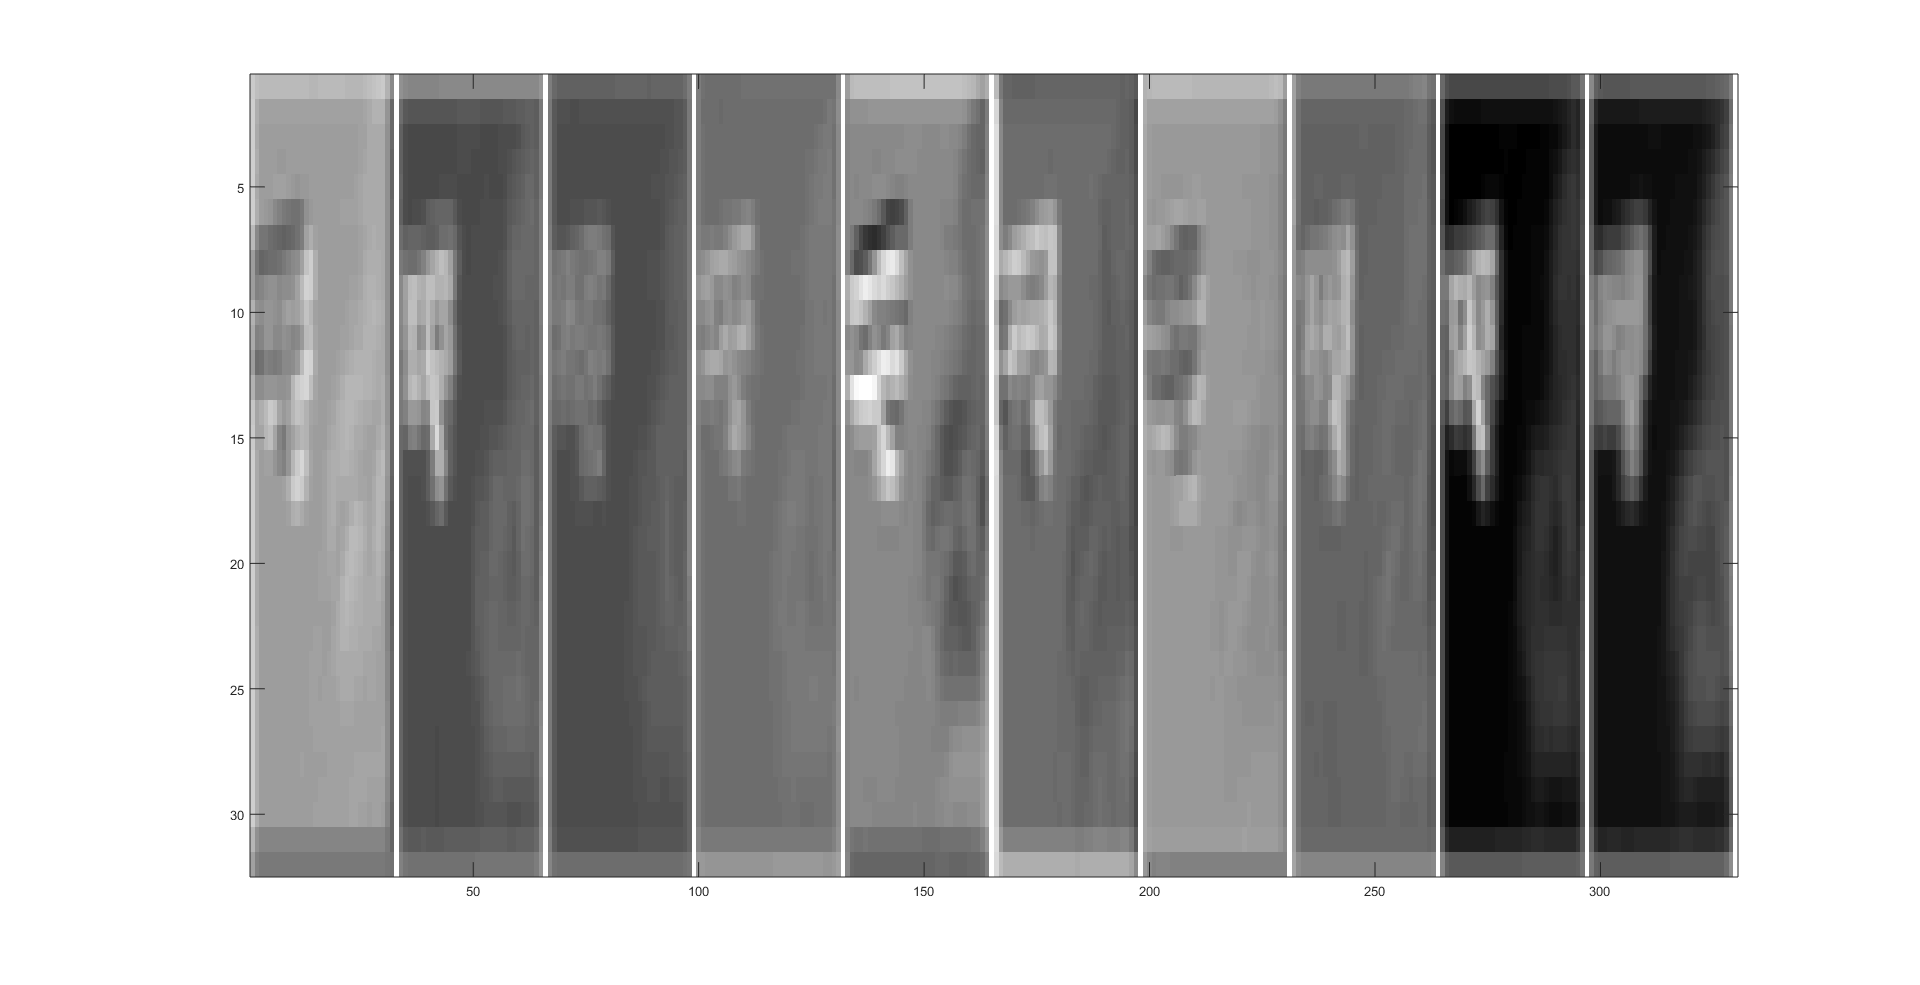
\includegraphics[width=\textwidth]{layer/4}
\end{figure}

\begin{figure}[h!]
  \caption{Layer 5 Output}
  \centering
    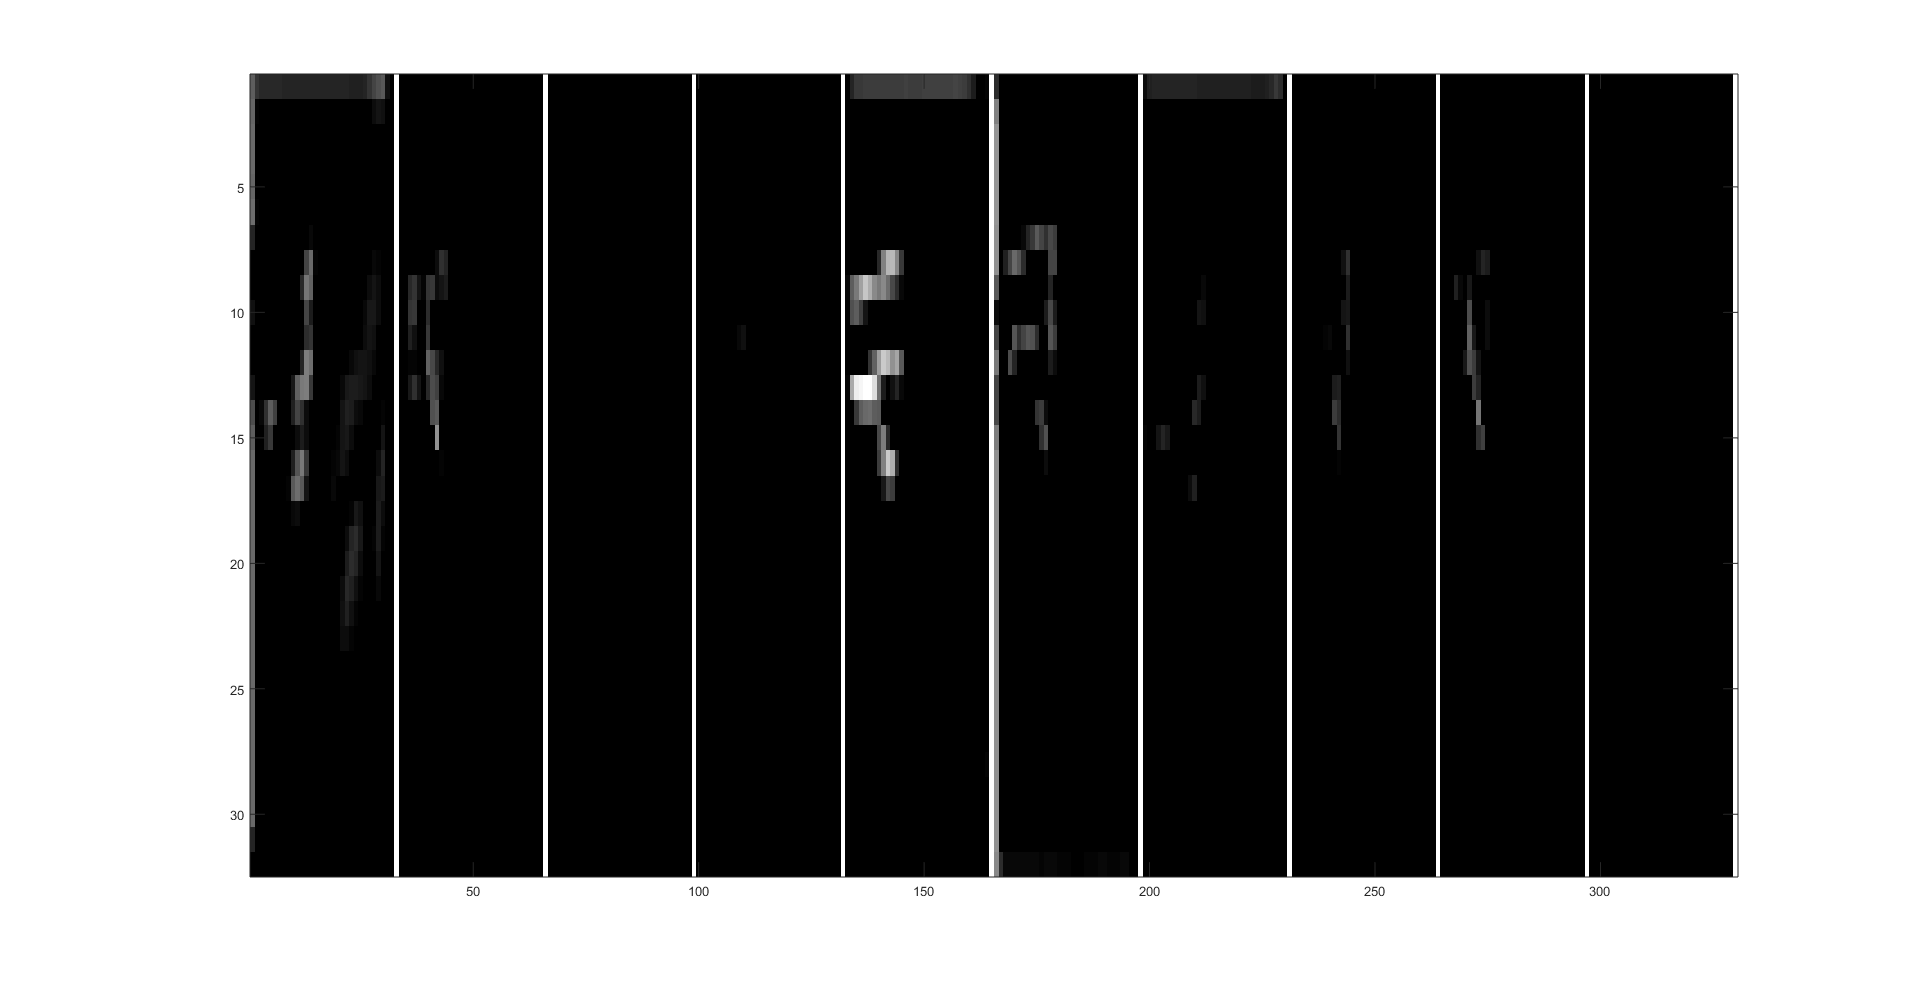
\includegraphics[width=\textwidth]{layer/5}
\end{figure}

\begin{figure}[h!]
  \caption{Layer 6 Output}
  \centering
    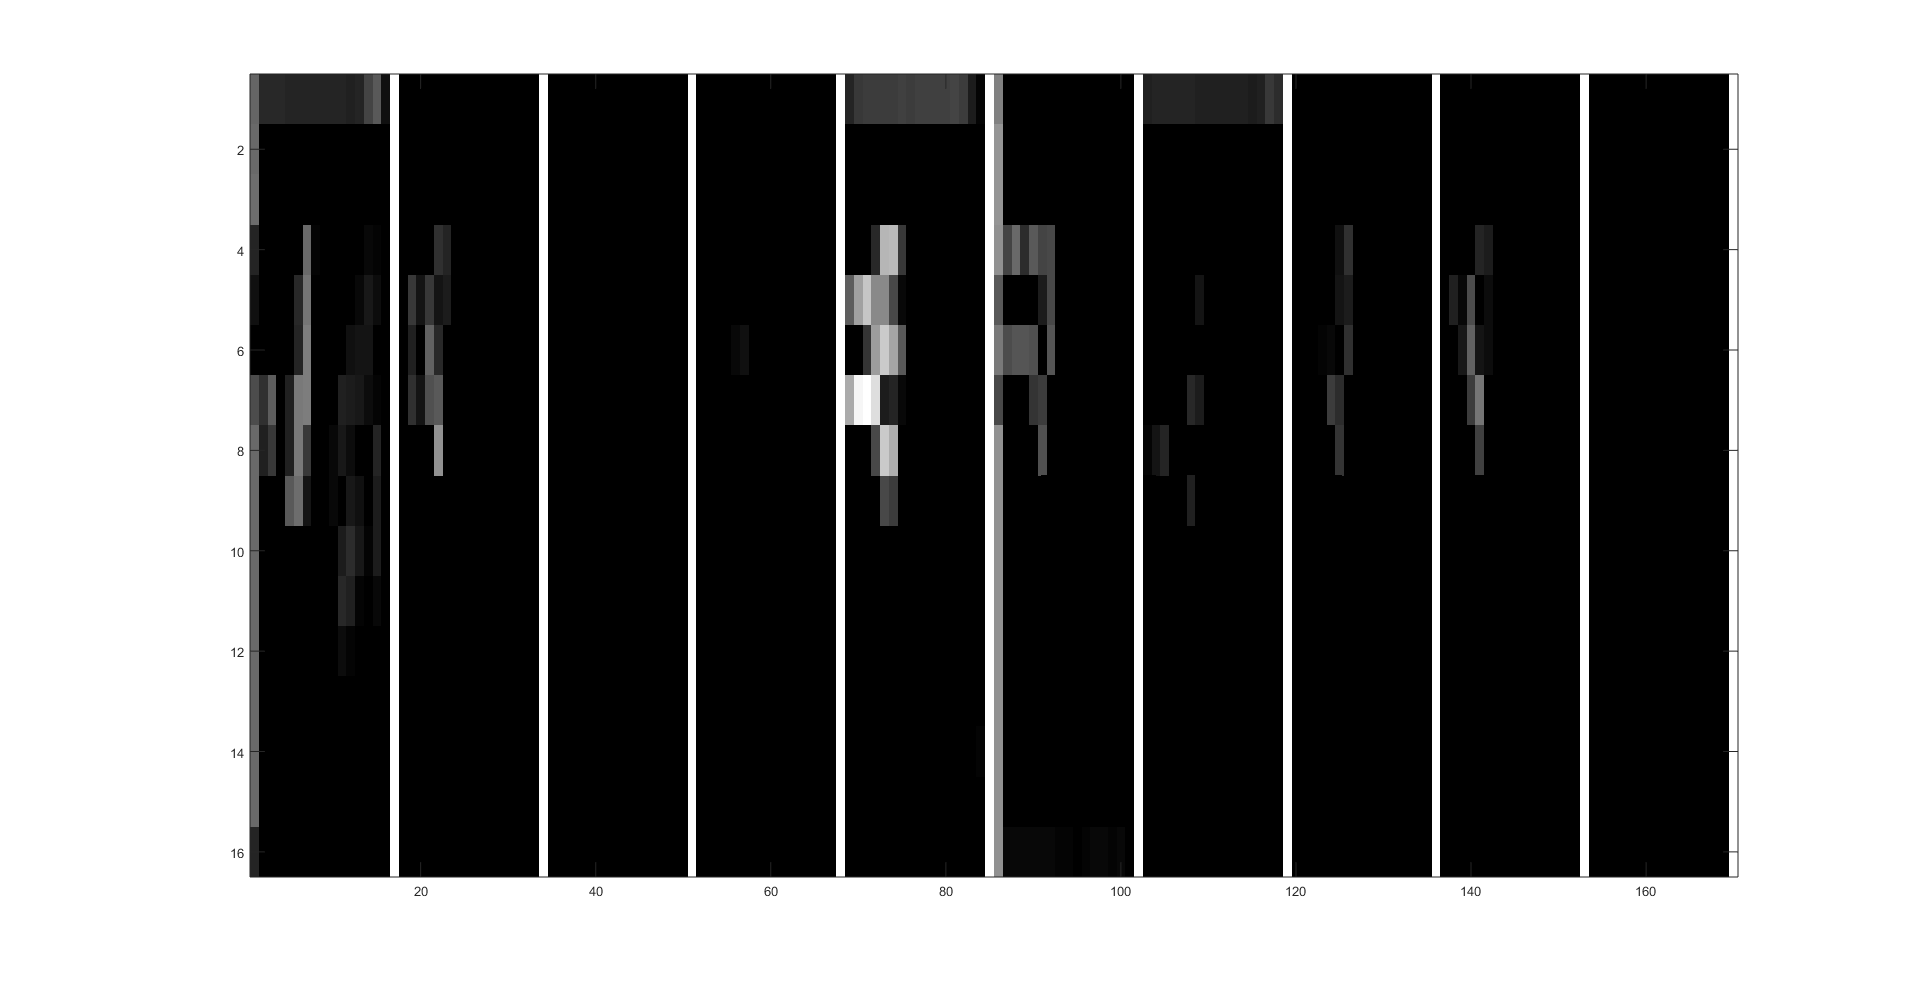
\includegraphics[width=\textwidth]{layer/6}
\end{figure}

\begin{figure}[h!]
  \caption{Layer 7 Output}
  \centering
    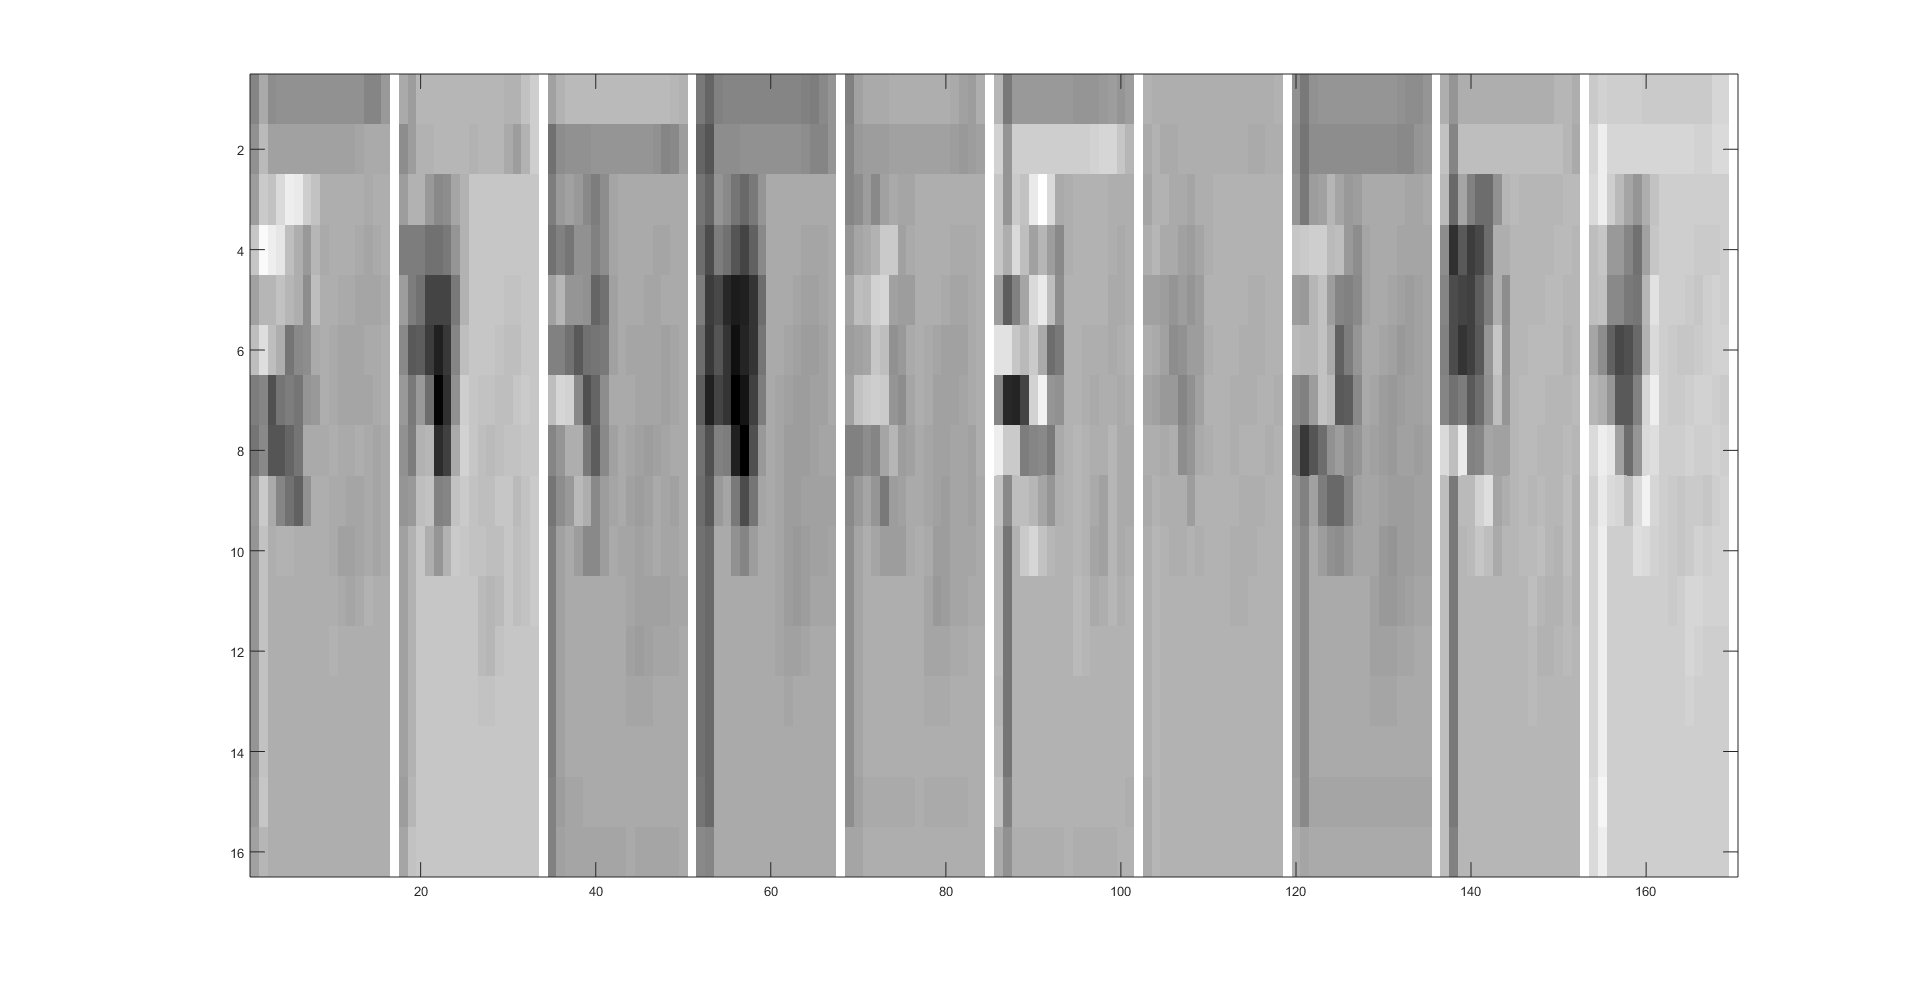
\includegraphics[width=\textwidth]{layer/7}
\end{figure}

\begin{figure}[h!]
  \caption{Layer 8 Output}
  \centering
    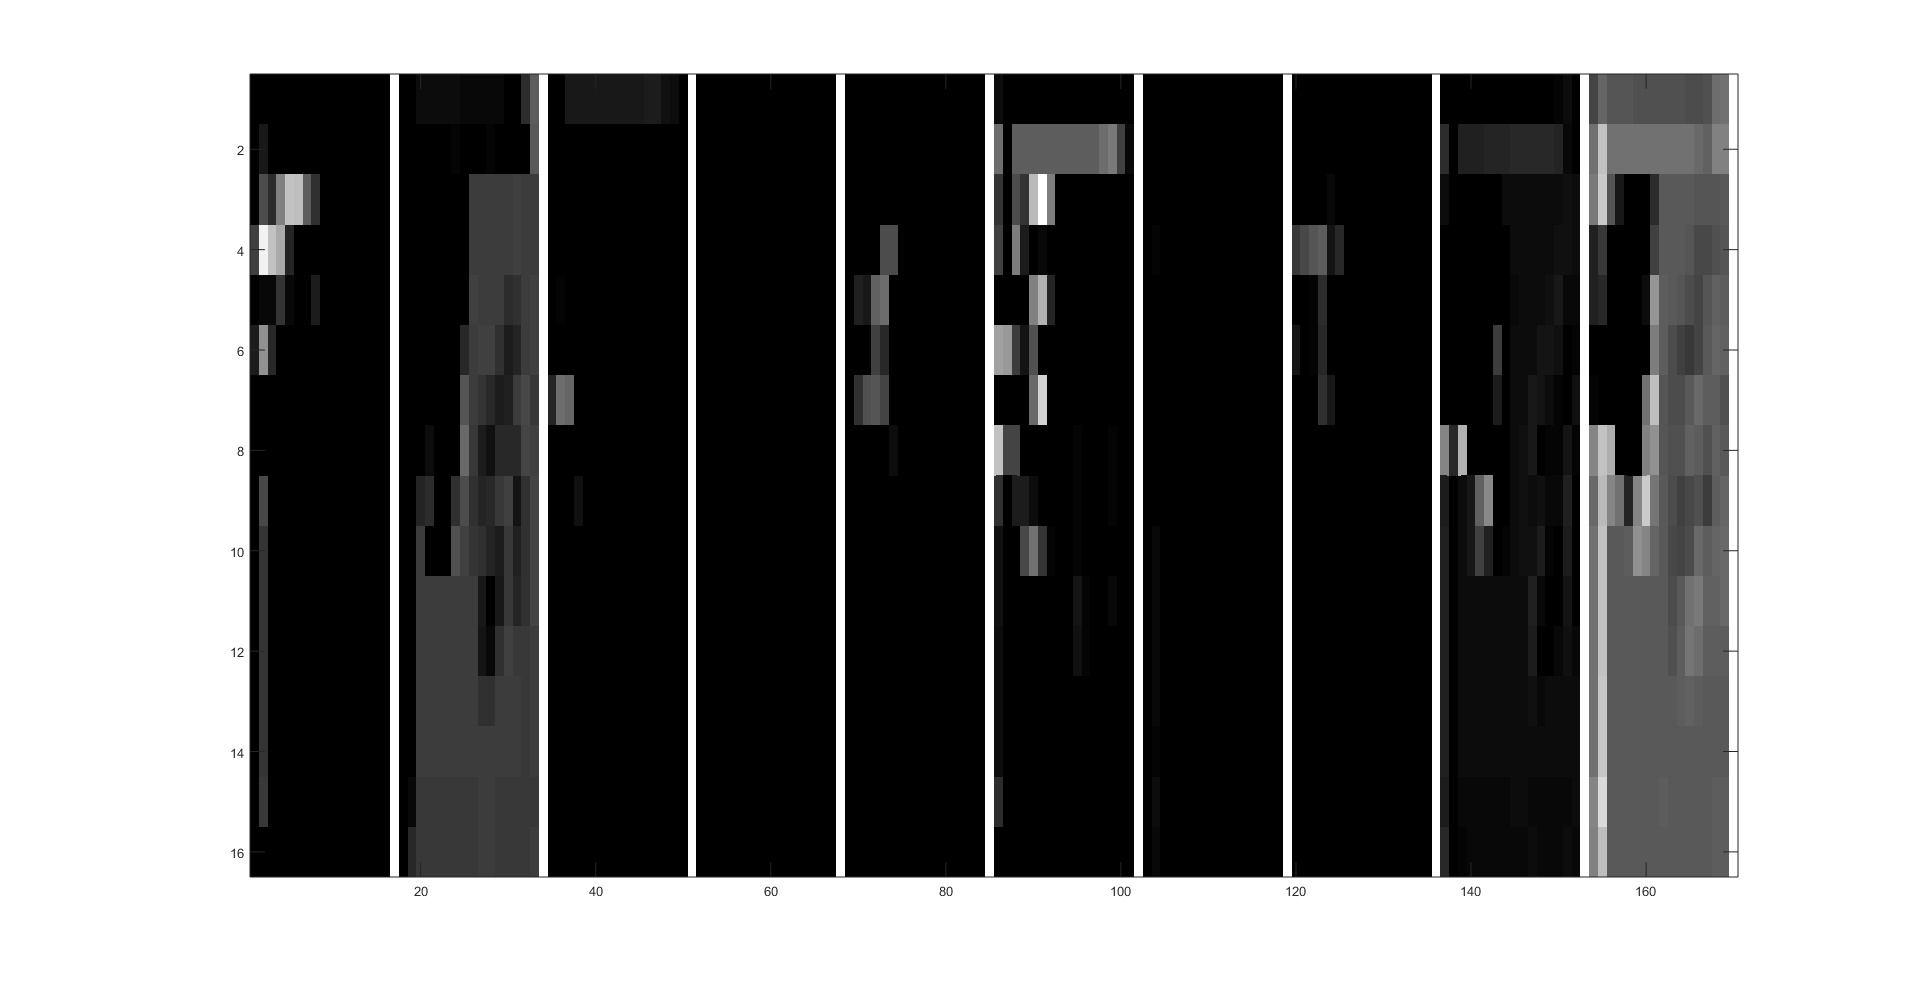
\includegraphics[width=\textwidth]{layer/8}
\end{figure}

\begin{figure}[h!]
  \caption{Layer 9 Output}
  \centering
    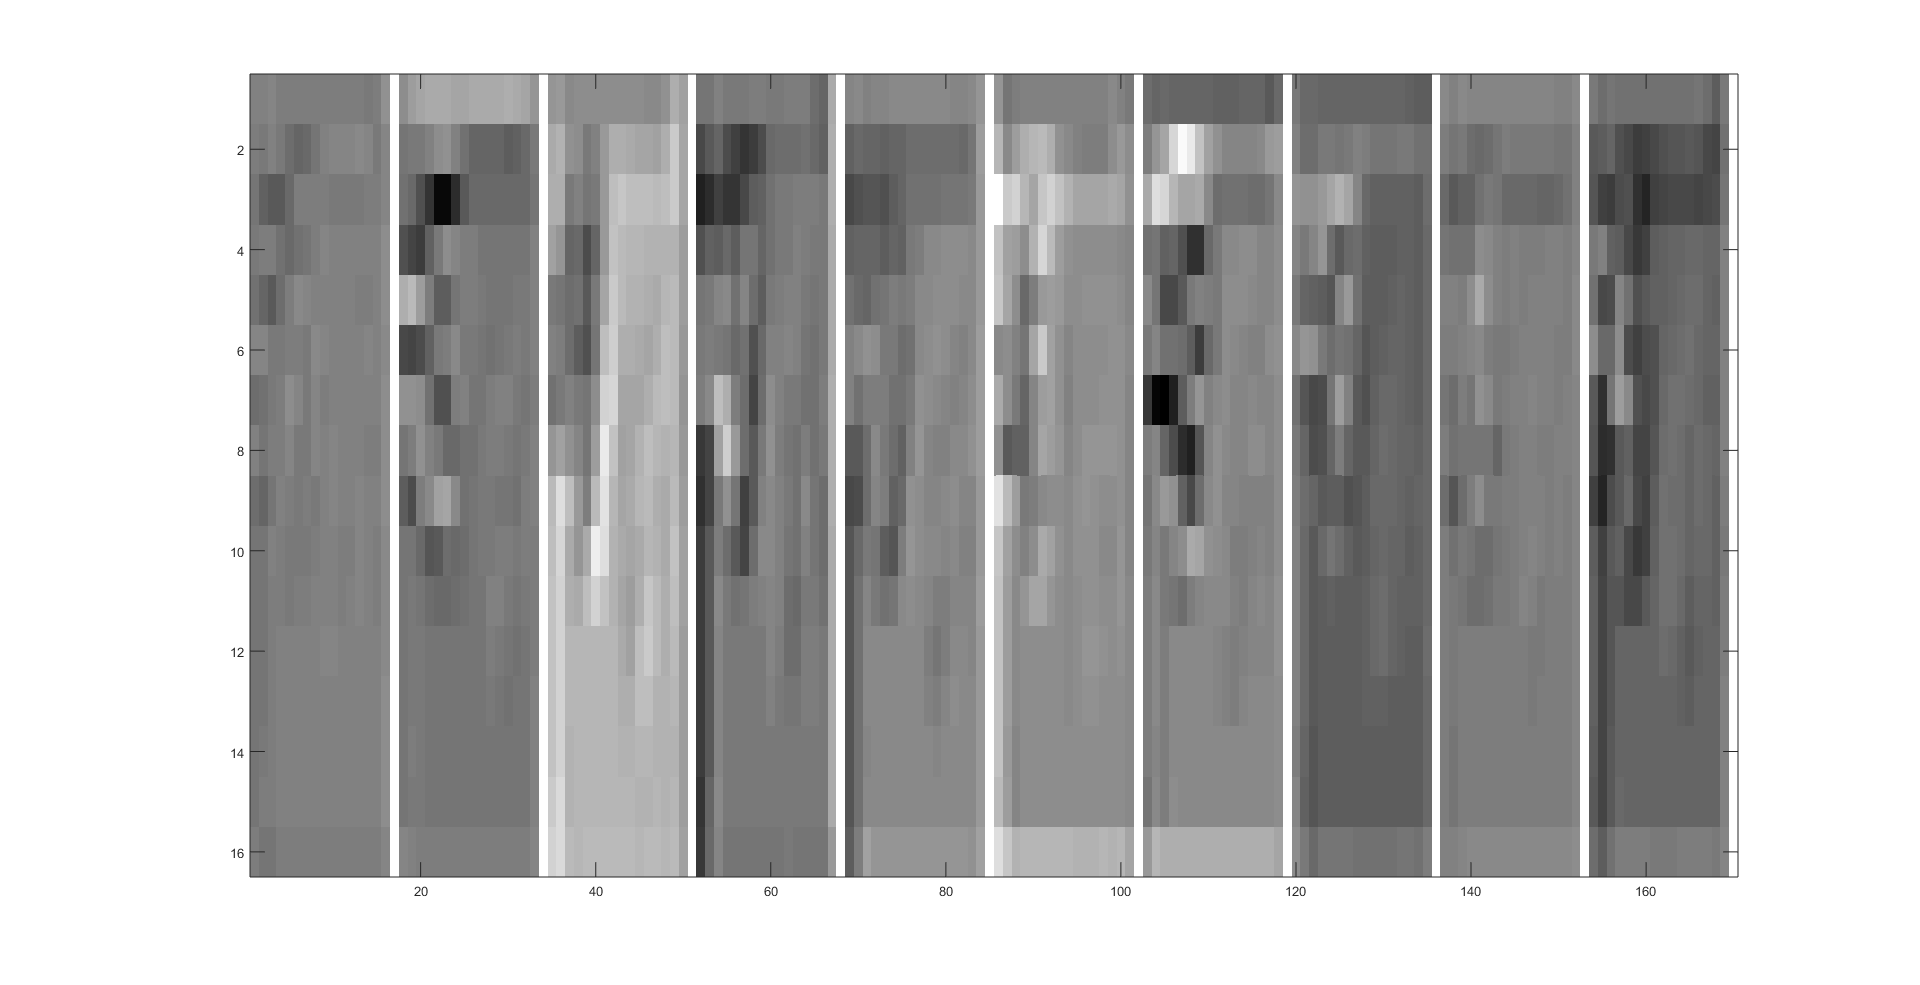
\includegraphics[width=\textwidth]{layer/9}
\end{figure}

\begin{figure}[h!]
  \caption{Layer 10 Output}
  \centering
    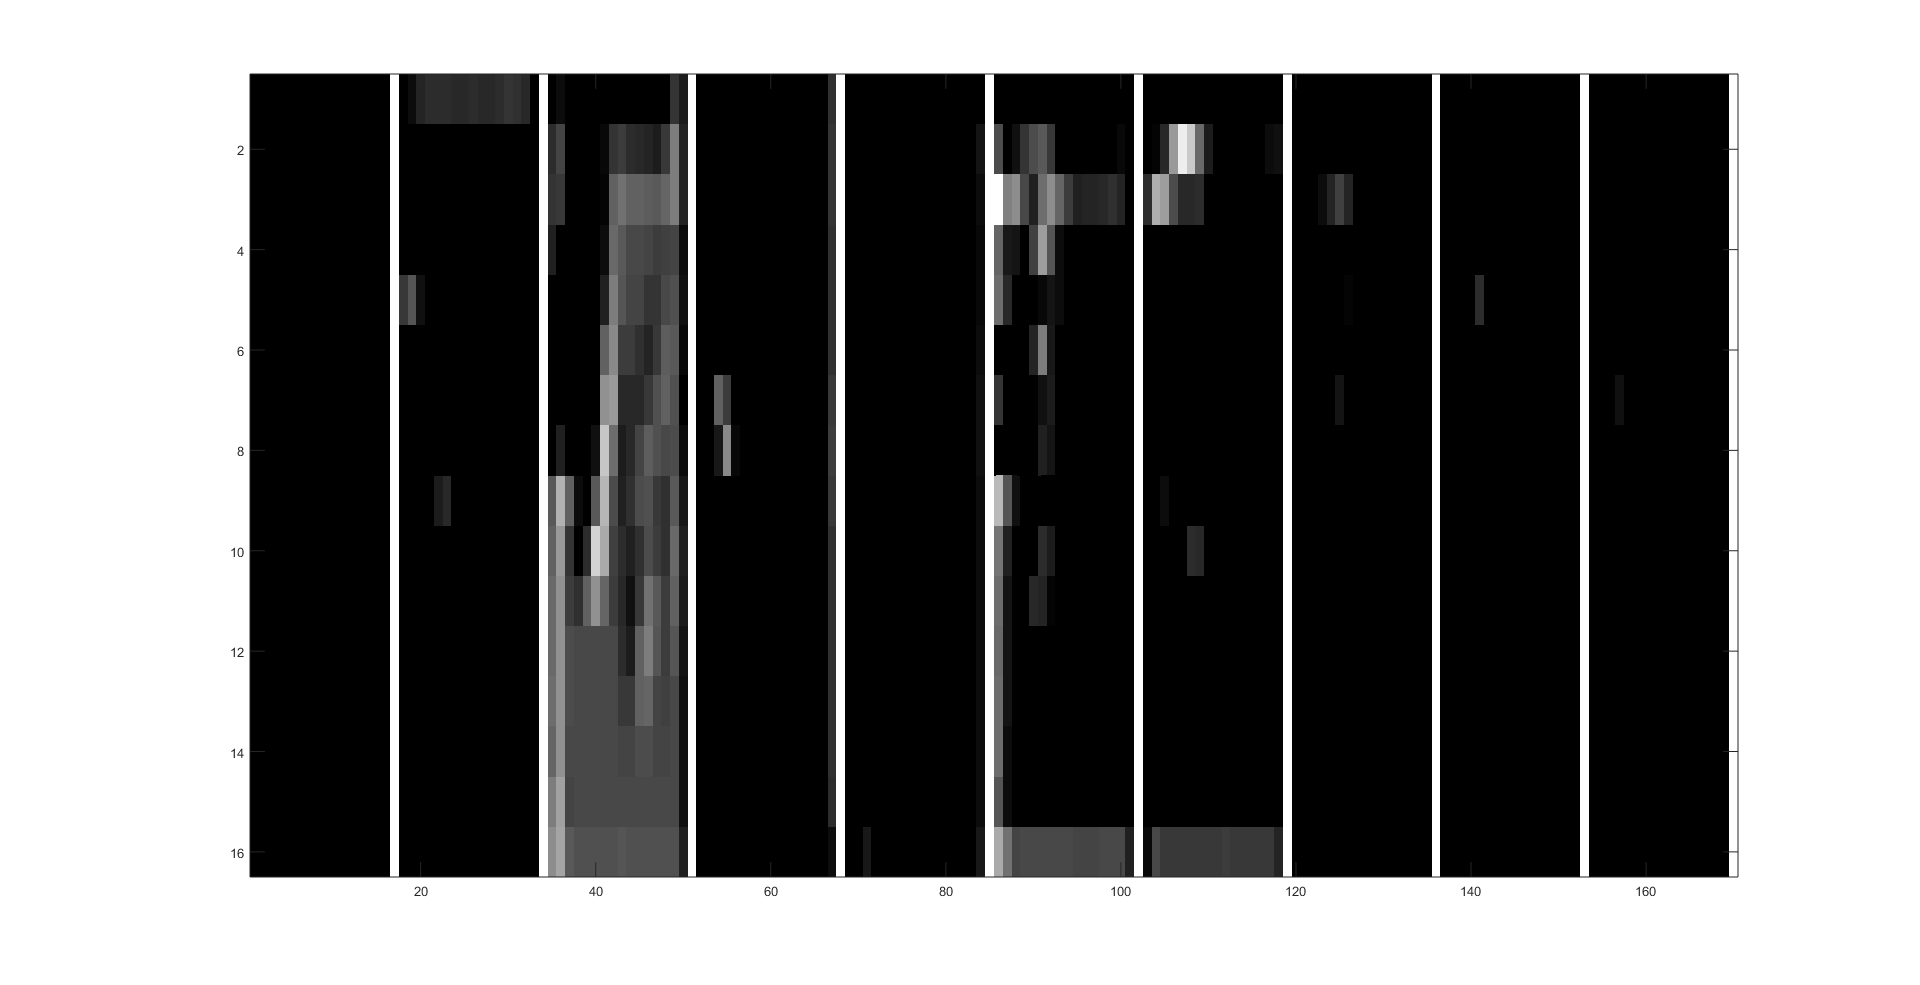
\includegraphics[width=\textwidth]{layer/10}
\end{figure}

\begin{figure}[h!]
  \caption{Layer 11 Output}
  \centering
    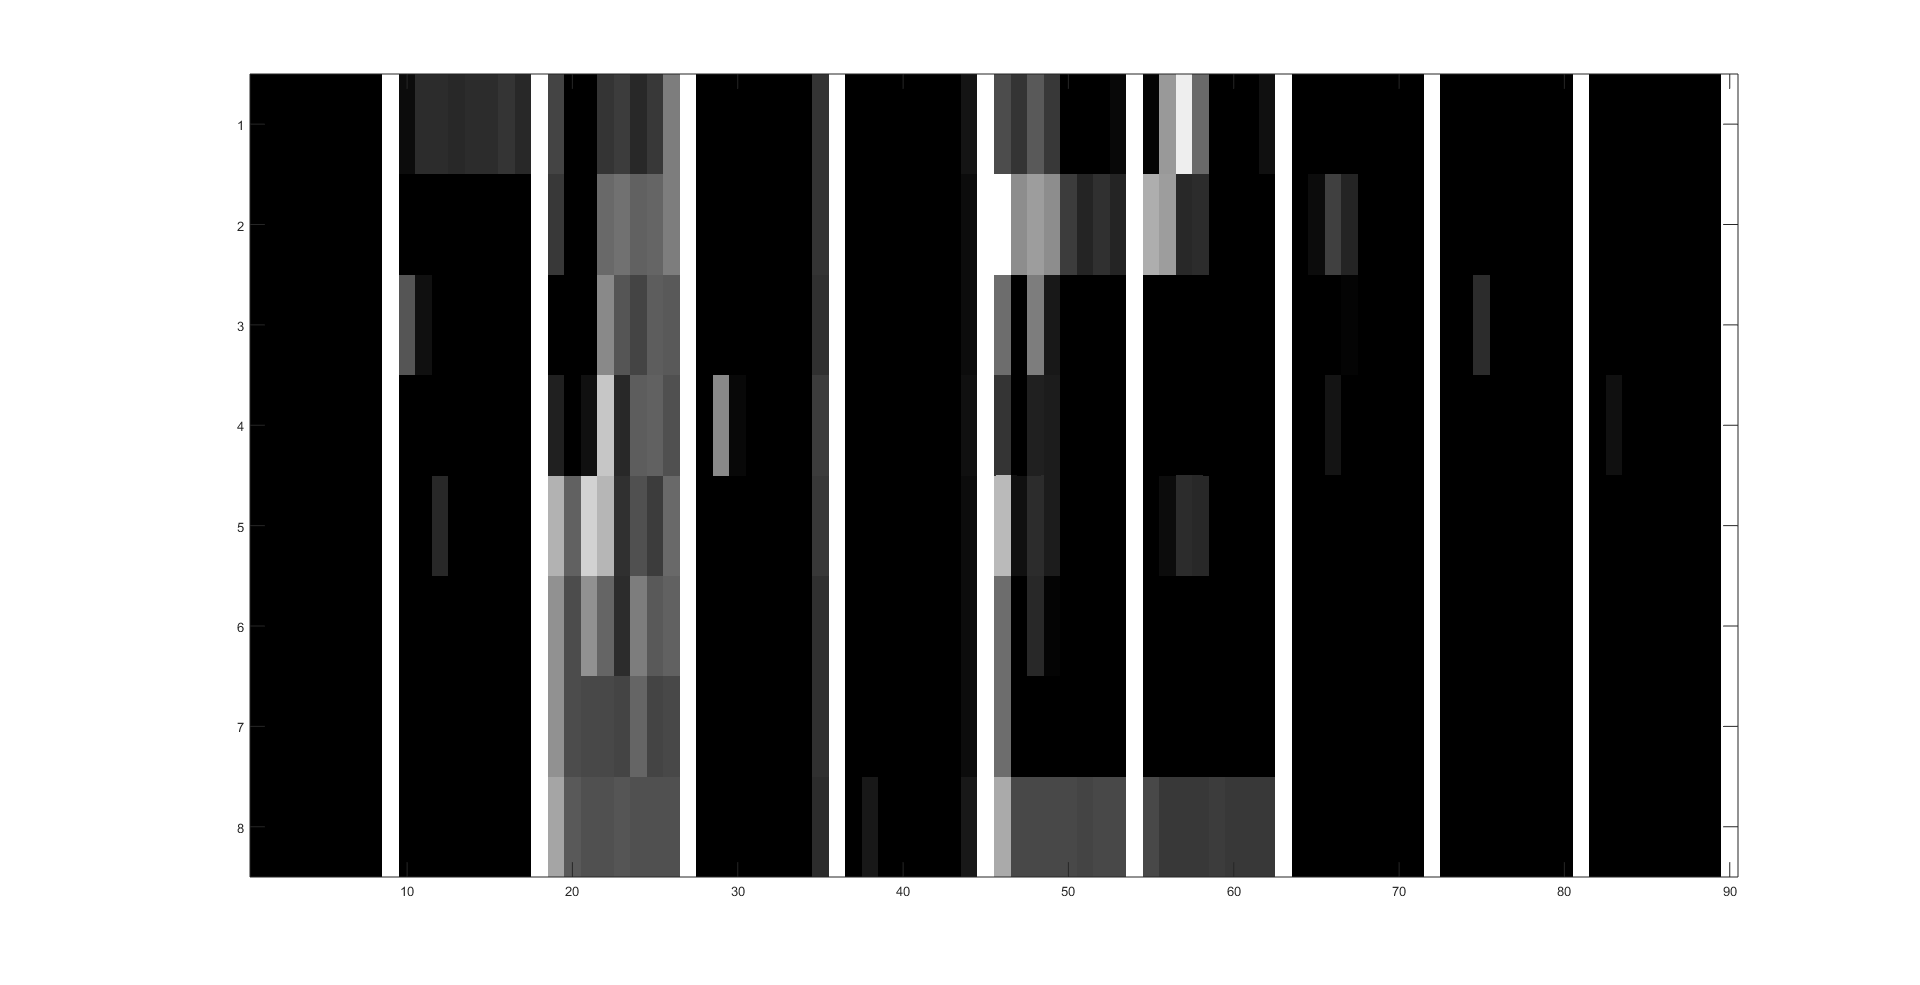
\includegraphics[width=\textwidth]{layer/11}
\end{figure}

\begin{figure}[h!]
  \caption{Layer 12 Output}
  \centering
    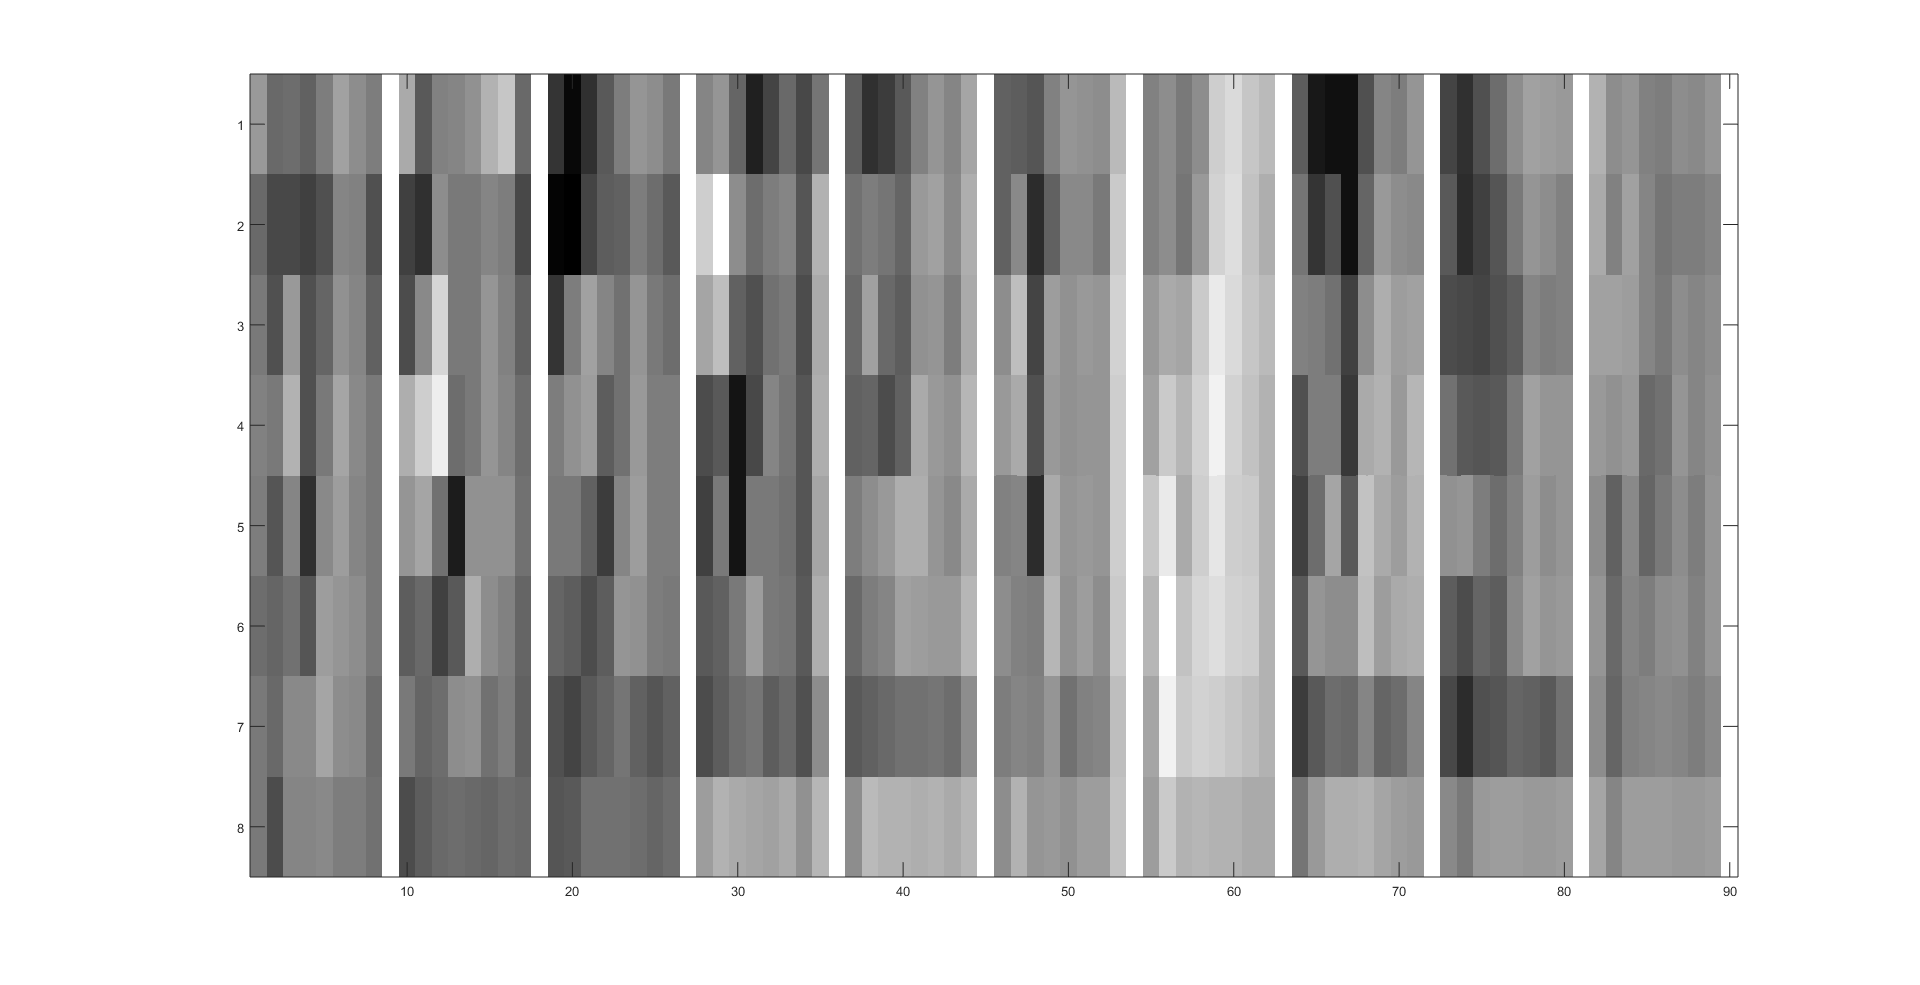
\includegraphics[width=\textwidth]{layer/12}
\end{figure}

\begin{figure}[h!]
  \caption{Layer 13 Output}
  \centering
    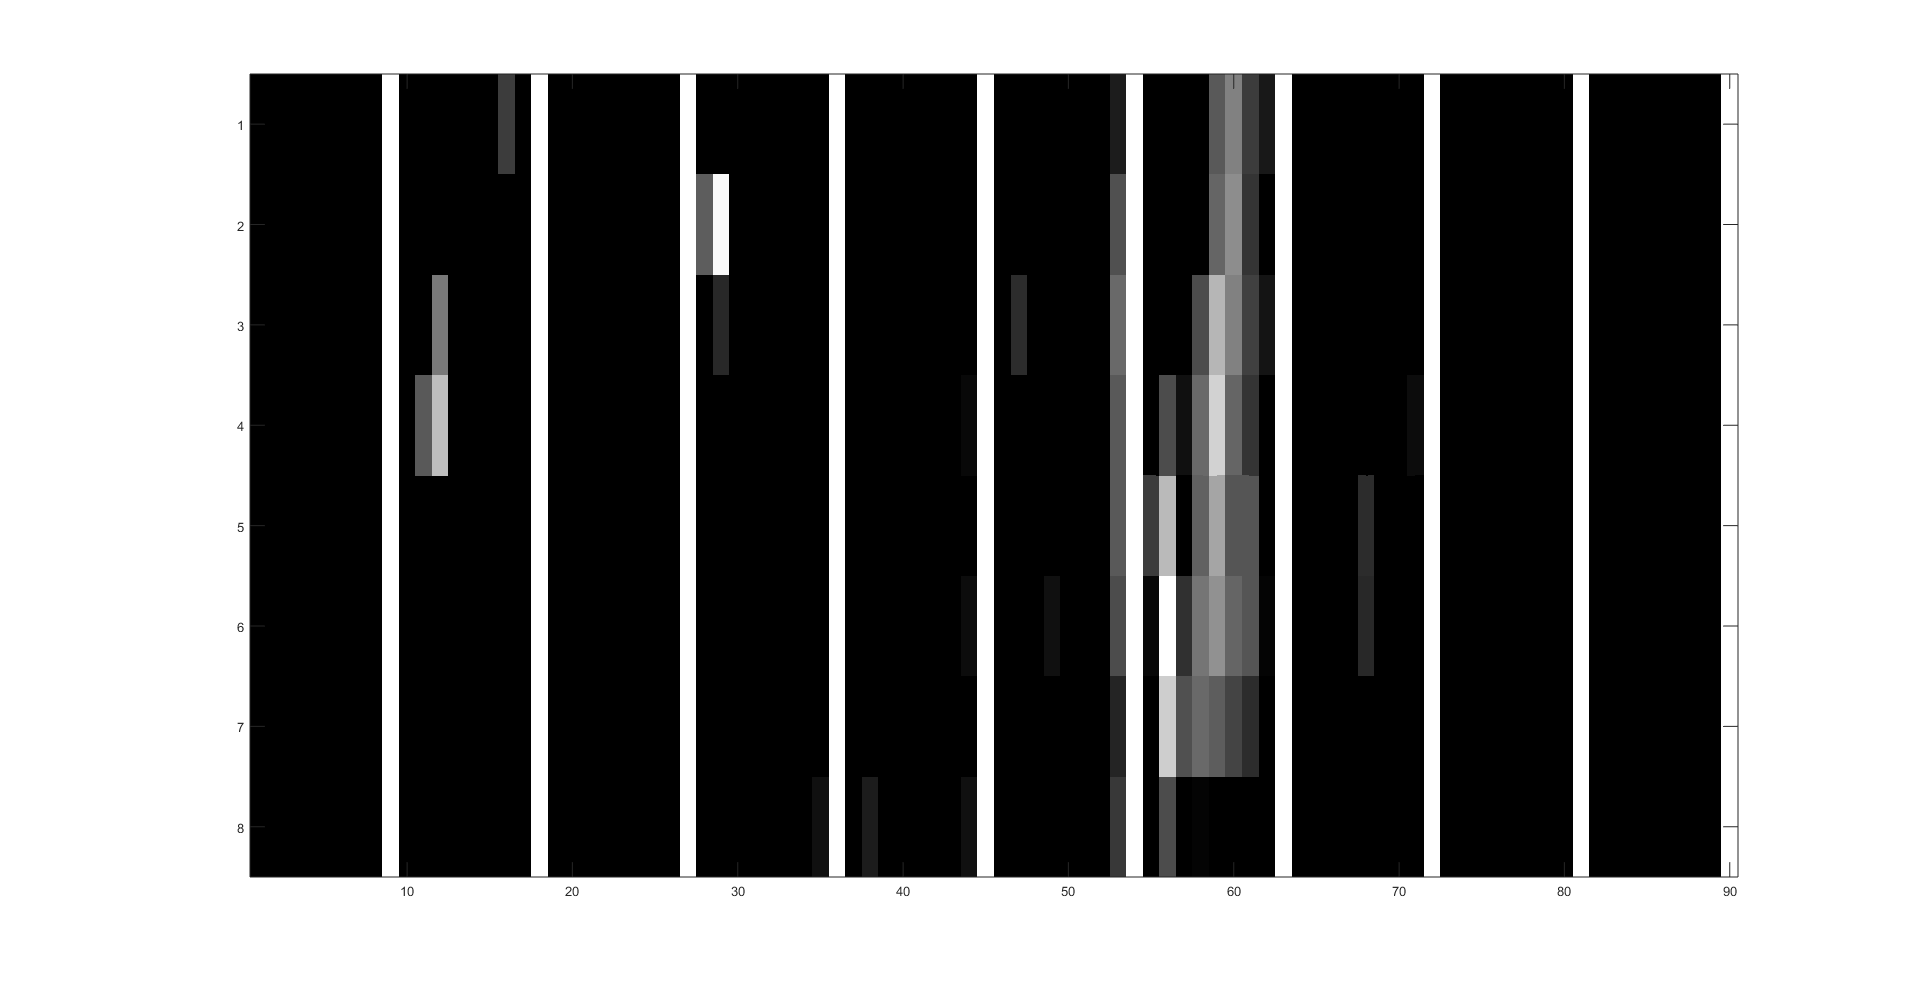
\includegraphics[width=\textwidth]{layer/13}
\end{figure}

\begin{figure}[h!]
  \caption{Layer 14 Output}
  \centering
    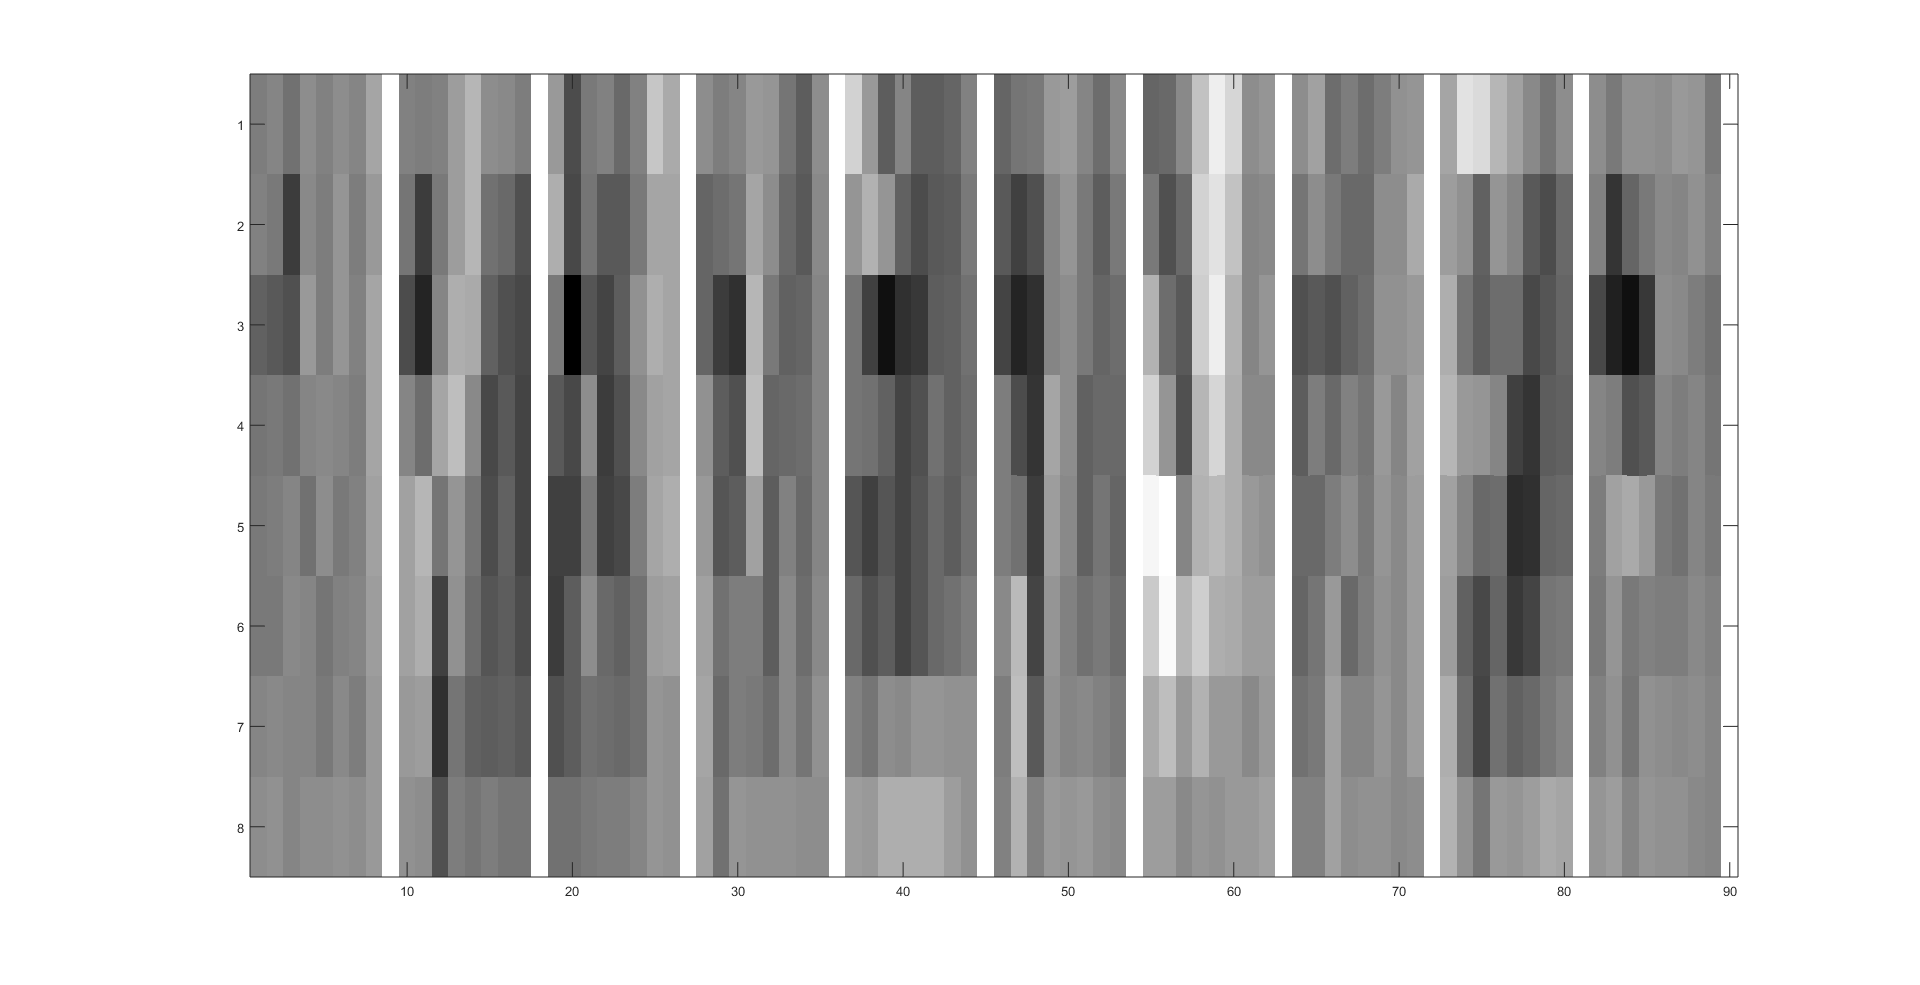
\includegraphics[width=\textwidth]{layer/14}
\end{figure}

\begin{figure}[h!]
  \caption{Layer 15 Output}
  \centering
    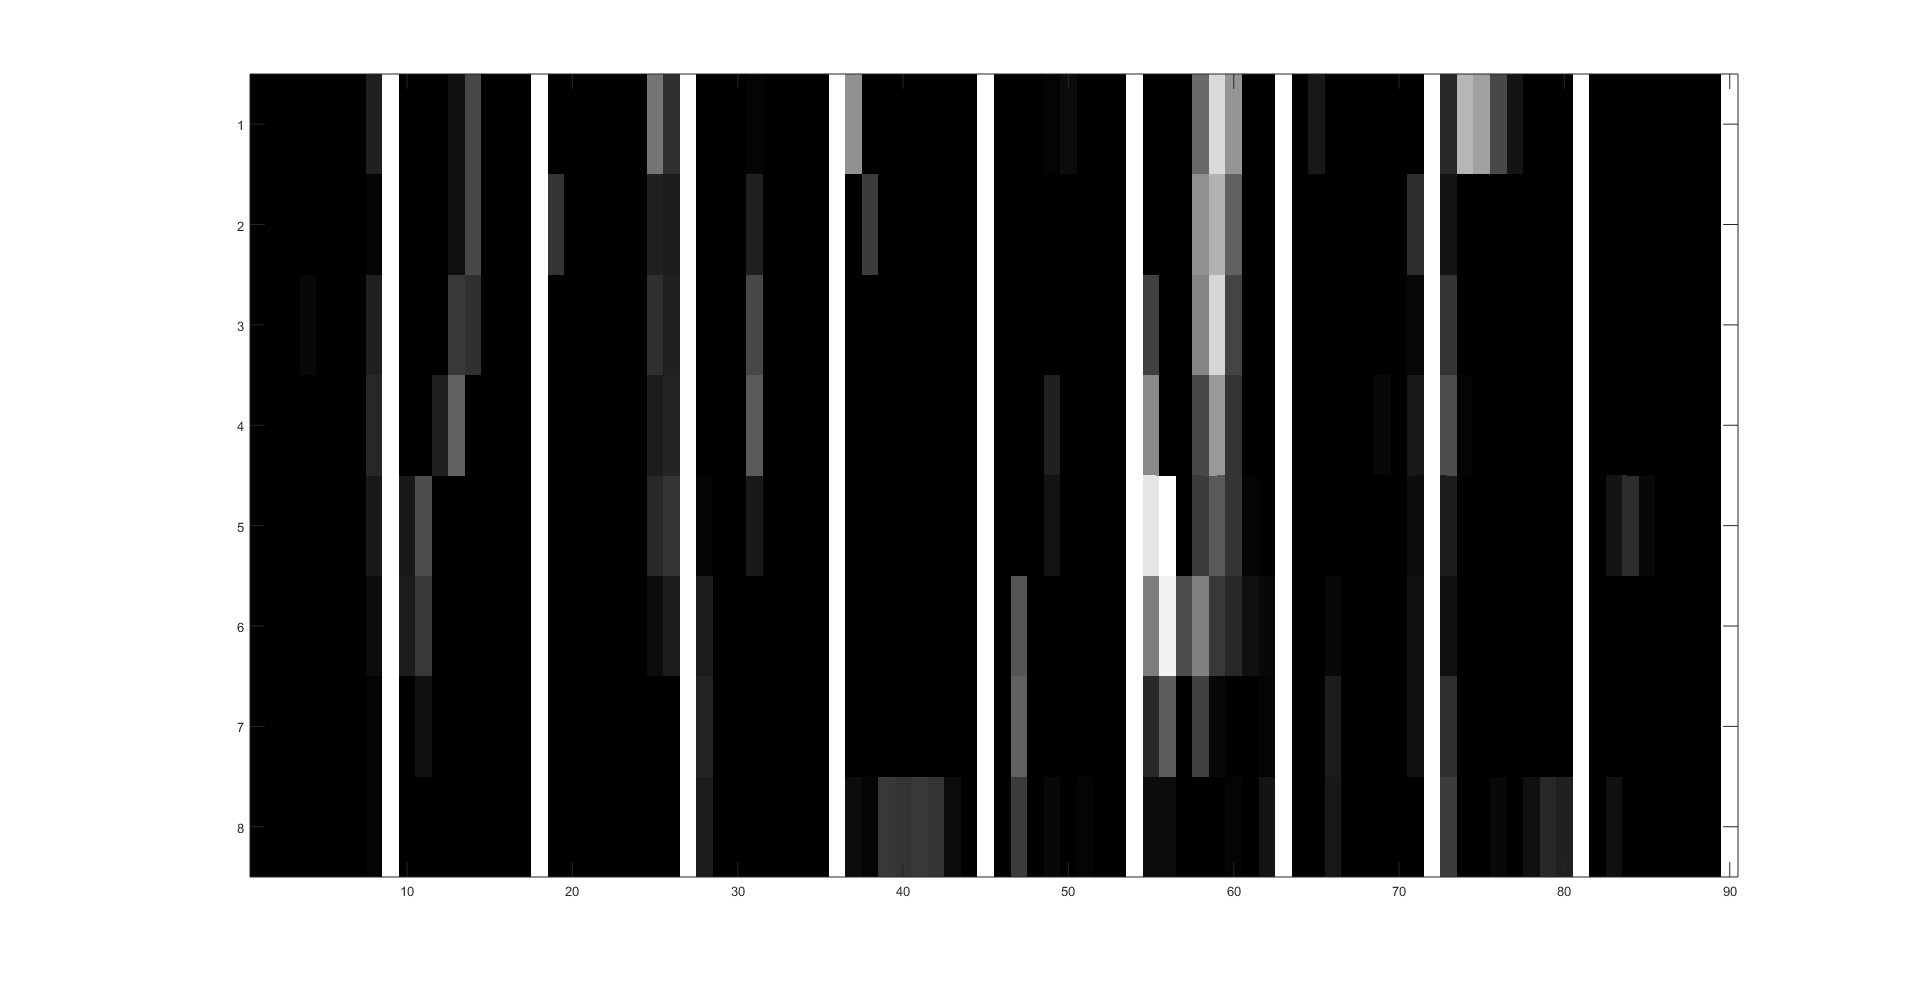
\includegraphics[width=\textwidth]{layer/15}
\end{figure}

\begin{figure}[h!]
  \caption{Layer 16 Output}
  \centering
    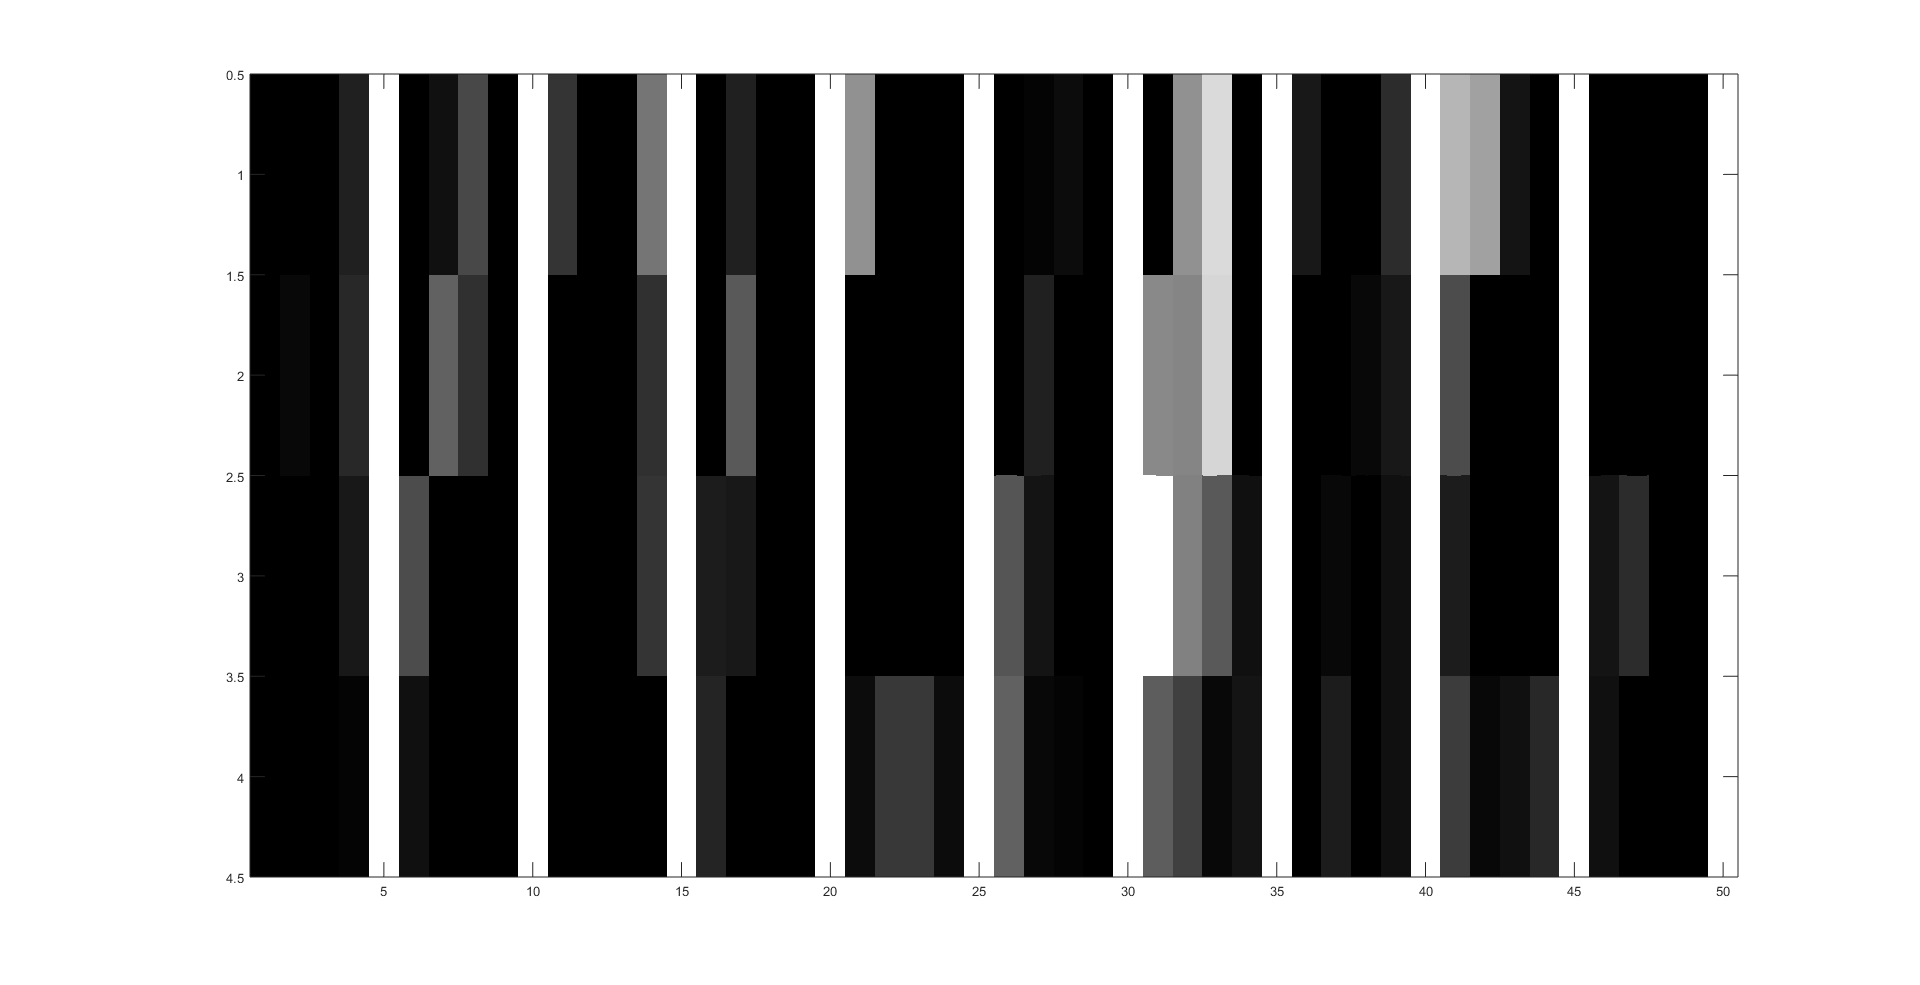
\includegraphics[width=\textwidth]{layer/16}
\end{figure}

\begin{figure}[h!]
  \caption{Layer 17 Output}
  \centering
    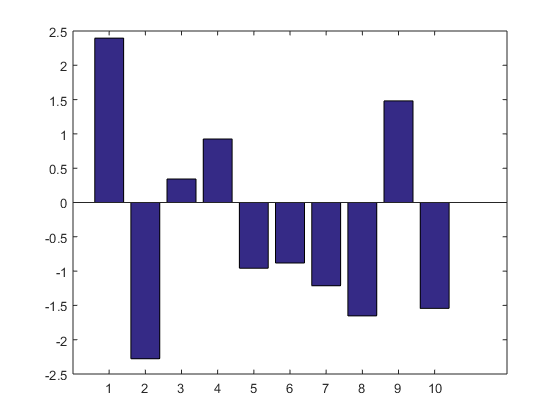
\includegraphics[width=0.75\textwidth]{layer/17}
\end{figure}

\begin{figure}[h!]
  \caption{Layer 18 Output}
  \centering
    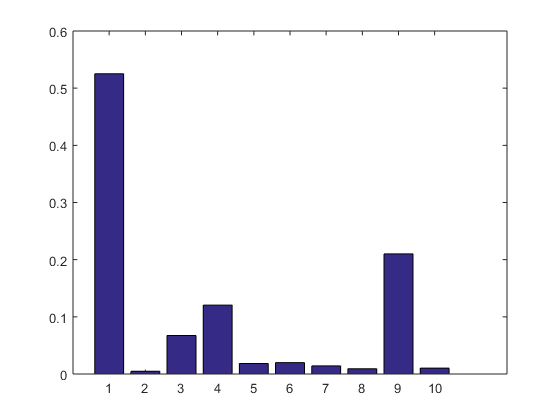
\includegraphics[width=0.75\textwidth]{layer/18}
\end{figure}


\end{appendices}

\end{document}